
% JuliaCon proceedings template
\documentclass{juliacon}
\setcounter{page}{1}

% Packages added to the template
\usepackage{subfig}
\usepackage{amsmath}
\usepackage{tikz}
\usepackage{cite}

\begin{document}

% **************GENERATED FILE, DO NOT EDIT**************

\title{My JuliaCon proceeding}

\author[1]{1st author}
\author[1, 2]{2nd author}
\author[2]{3rd author}
\affil[1]{University}
\affil[2]{National Lab}

\keywords{Julia, Optimization, Game theory, Compiler}

\hypersetup{
pdftitle = {My JuliaCon proceeding},
pdfsubject = {JuliaCon 2019 Proceedings},
pdfauthor = {1st author, 2nd author, 3rd author},
pdfkeywords = {Julia, Optimization, Game theory, Compiler},
}



\maketitle

\begin{abstract}

    This paper introduces a modeling and simulation framework, Causal.jl,  that enables fast and effective system simulations and online and offline data analyzes. Causal.jl adopts a causal modeling approach in which a model consists of components that process data and the connections that transfer the data flowing between these components. The framework developed makes it possible to simulate discrete time or continuous time, static or dynamical systems. In particular, it is possible to simulate dynamical systems modeled by various types of equations such as the ordinary, random ordinary, stochastic, delayed differential, differential-algebraic equations, and discrete-time difference equations. During the simulation, the data flowing through the connections can be processed online and offline, and specialized analyzes can be performed. These analyzes can also be enriched with plugins that can be easily defined using the standard Julia library or various Julia packages. The simulation is performed by evolving the model components between sampling time intervals individually and in parallel. The independent evolution of the components allows the simulation of the models consisting of the components represented by different mathematical equations, while the parallel evolution of components increases the simulation performance.

\end{abstract}

\section{Introduction}

Numerical simulations can be expressed as solving the mathematical equations derived from modeling physical systems. Based on the system's properties at hand and abstraction level in the modeling, mathematical equations may be ordinary, stochastic, delay differential, or difference equations. High-speed performance and the ability to offer useful analysis tools are other typical features expected from an effective simulation environment.

Many simulation environments are available for numerical analysis of systems\cite{elmqvist1978structured,nytsch2006advanced,zimmer2008introducing,mosterman2002hybrsim,van2001variables,giorgidze2009higher,pfeiffer2012pysimulator,simulink}. They are capable of allowing simulations that are represented by ordinary differential equations and differential algebraic equations, mostly. This is restrictive given the variety of mathematical equations that can be derived from the modeling\cite{rackauckas2017differentialequations}. Besides, many of the existing simulation environments lack modern computational methods such as parallel computing.

In this study, Causal.jl, a modeling and simulation framework for causal models, is introduced \cite{causal}. The aim is to model large scale complex system networks easily and to provide fast and effective simulations. For this purpose, Julia, an open-source, high level, general purpose dynamical programming language designed for high-performance numerical analysis and computational science, has been used. Although Julia is a dynamical language, owing to its Just-in-Time(JIT) compiler developed on Low Level Virtual Machine(LLVM), it can reach the high-speed performance of static languages such as C\cite{bezanson2017julia,julialang}. It supports various parallel computing techniques at thread and process levels. In addition to Julia's standard library, numerous specialized packages developed for different fields such as data science, scientific computing, are also available. Julia's high-speed performance and parallel computing support are essential in meeting the need to design a  fast and effective simulation environment. Julia's syntax can be enlarged purposefully using its metaprogramming support. The analyzes scope of the simulation framework can be extended with new plugins that can be easily defined. It is possible to analyze discrete or continuous-time, static, or dynamical systems. In particular, it is possible to simulate dynamical systems modeled by ordinary, random ordinary, stochastic, delay differential, differential-algebraic, and/or discrete difference equations simultaneously. Unlike its counterparts, the models do not evolve at once for the whole simulation duration. Instead, the model components evolve between sampling time intervals individually. While individual evolution of the components enables the simulation of systems consisting of components represented by different mathematical models, parallel evolution of components increases the simulation performance.




\section{Modeling and Simulation}

\subsection{Modeling}
Causal.jl adopts causal modeling\footnote{Causal modeling is also known as signal flow modeling or block diagram modeling} approach in modeling systems. In causal modeling approach, a model consists of components and connections (Figure \ref{fig: simple model})\cite{matei2012modeling}. The simulation of the model is performed in a clocked environment. That is, the model is not simulated in one shot by solving a single mathematical equation system that represents the whole model, but instead, it is simulated by evolving the components between sampling intervals in parallel, individually.

The components interact with each other through the connections that are bound to their input/output ports. The components are data processing agents, and their behavior determines how the data is processed. Depending upon the nature of the system and the modeling, these equations may differ, i.e., they may or may not contain derivative terms, or they may contain the continuous or discrete-time variable, etc. The dataflow through the connections is unidirectional, i.e., a component is driven by other components that write data to its input port.

The model simulation is performed by evolving the components individually. A reference clock is used to make the components have a common time base. The clock generates pulses at simulation sampling intervals. These pulses are used to trigger the components during the run stage of the simulation. Each triggered component reads its input data from its input port, calculates its output according to its mathematical model, and writes the result to its output port.

\begin{figure}
    \centering
    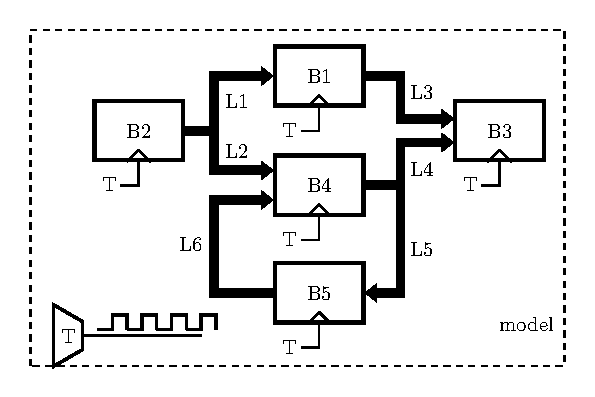
\includegraphics[width=0.75\linewidth]{figures/Model/model.pdf}
    \caption{A model consisting of the components B1, $\ldots$, B5 and the connections L1, $\ldots$, L6. T is the common time reference of the model.}
    \label{fig: simple model}
\end{figure}

\subsection{Components}

The component types in Causal.jl are shown in Figure \ref{fig: component types}. The components can be classified as sources, sinks, and systems.

The sources are the components that generate outputs as functions of time only. When triggered, a source computes its output according to its readout function and writes the result to its output port. The sources do not have input ports.

The sinks are data processing units. Their primary goal is to process the data flowing through the connections online. When triggered, a sink reads its input data from its input port and processes it. The data can be visualized by being plotted on a graphical user interface, can be observed by being printed on a console, or can be recorded in data files. The sinks' data processing scope can be enriched by integrating new plugins that can be developed using the standard Julia library or various available Julia packages. Invariants, spectral properties, or statistical information can be extracted from the data. Parameter estimation can be performed, or various signal processing techniques can be applied. Causal.jl has been designed to be flexible enough to allow the users to extend its data analyzes scope by integrating newly-defined plugins.

\begin{figure}
    \centering
    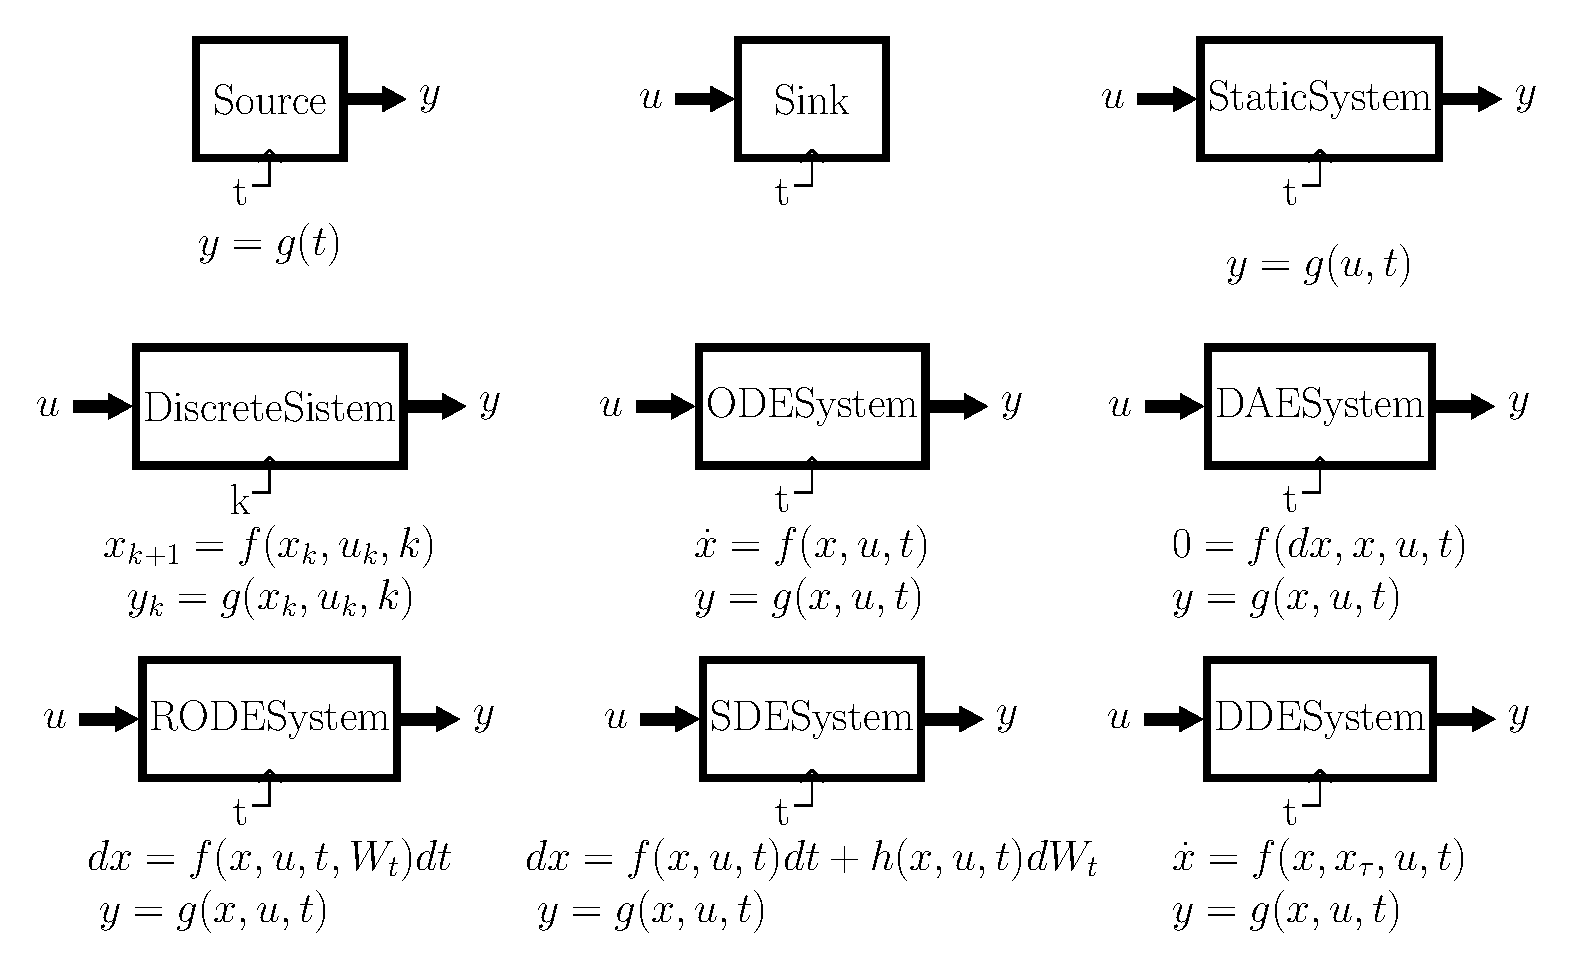
\includegraphics[width=\linewidth]{figures/ComponentsCompressed/components_compresses.pdf}
    \caption{Component types in Causal.jl. $u, x, y$ signify the input, state, output of a system, respectively. $t$ and $k$ are continuous and discrete time variable, respectively. $W$ is the stochastic process corresponding to the noise and $x_\tau$ is the state $x$ delayed by $\tau$ seconds in time. $f$(and $h$) is the right-hand-side function of the differential equation representing the system and $g$ is the readout function.}
    \label{fig: component types}
\end{figure}

A static system is described by a readout equation solely. When triggered, a static system reads its input data from its input port, calculates its output according to its readout function, and writes the result to its output port. In dynamic systems, however, the system behavior is characterized by the states. The output of a dynamical system depends on its input, previous state(s), and time. Therefore, a dynamical system is described by a differential equation and a readout equation, classically. When triggered, a dynamical system reads its input from its input port, updates its state according to the differential equation, calculates its output according to its readout function, and writes the result to its output port. Being developed on top of DifferentialEquations.jl, Causal.jl is capable of simulating the dynamical systems represented by differential equations in the form of the ordinary differential equations(ODE), differential-algebraic equations(DAE), random ordinary differential equations(RODE), stochastic differential equations(SDE), delay differential equations(DDE) or discrete difference equations \cite{rackauckas2017differentialequations}. Most of the available simulation environments allow the systems represented by ordinary differential equations or differential-algebraic equations\cite{elmqvist1978structured,nytsch2006advanced,zimmer2008introducing,mosterman2002hybrsim,van2001variables,giorgidze2009higher,pfeiffer2012pysimulator,simulink}. Therefore, analyzes such as noise or delay analysis or unexpected change of system parameters cannot be performed in these simulation environments, easily. On the contrary, Causal.jl makes it possible for all these analyses to be performed owing to its ability to solve such a wide range of differential equations.

\subsection{Ports and Connections}
A port is a bunch of pins to which the connections are bound. There are two types of pins: an output pin that transfers data from the inside of the component to its outside, and an input pin that transfers data from the outside of the component to its inside. There are two types of ports: an output port that consists of output pins and an input port that consists of input pins.

\begin{figure}
    \centering
    \subfloat[]{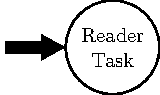
\includegraphics[width=0.225\linewidth]{figures/Tasks/reader_task.pdf} \label{subfig: reader task}} \hfil 
    \subfloat[]{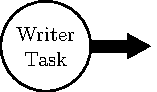
\includegraphics[width=0.225\linewidth]{figures/Tasks/writer_task.pdf} \label{subfig: writer task}} \hfil 
    \subfloat[]{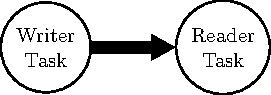
\includegraphics[width=0.4\linewidth]{figures/Tasks/reader_writer_task.pdf} \label{subfig: reader writer task}} 
    \caption{\protect\subref{subfig: reader task} A readable connection, \protect\subref{subfig: writer task} A writable connection, \protect\subref{subfig: reader writer task} A readable and writable connection}
    \label{fig: tasks}
\end{figure}

The data transferred to a port are transferred to its connections. The data transfer through the connections is performed over the links of the connections. The links are built on top Julia channels. The data written to(read from) a link is written to(read from) its channel. Running Julia tasks bound to the channels must exist for the data to flow through these channels. Julia tasks are the control flow features that allow calculations to be flexibly suspended and maintained without directly communicating the task scheduler of the operating system\cite{julialang}. The communication and the data exchange between the tasks are carried out through Julia's channels to which they are bound.

Figure \ref{fig: tasks} depicts the tasks that must be bound to a connection to make it readable, writable, and both readable and writable, symbolically. The writer(the reader) task is the task that writes(reads) data to(from) the connection. A running writer task must be bound to the connection on the opposite side to read data from one side of a connection. This connection is called a readable connection. Similarly, to write data to one side of a connection, a running reader task must be bound to the connection at the other side. This connection is called a writable connection. If both running writer and reader tasks are bound to both sides of a connection, then the data can both be read from and written to the connection. Such a connection is called a readable and writable connection. The dataflow through a connection is only allowed if the connection is both readable and writable connection. The data read from a readable connection is the data written to the connection by the writer task of the connection. If the data have not been written to the connection by its writer task during a reading process yet, then reading does not occur, and the writer task is waited to put data to the connection. Similarly, if the data on a connection has not been read from the connection by its reader task during a writing process yet, then the reader task is waited to take data from the connection.

In the modeling approach adopted, the components reading data from a connection are driven by other components writing data to the connection. Therefore, all of the model's connections must be readable and writable so that data can flow through the connections. This necessitates that all the connections of the model must be connected to a component from both ends. Otherwise, the simulation gets stuck and does not terminate.

\subsection{Simulation}
A model to be simulated consists of components connected to each other and a time reference. The time reference is used to sample the continuous-time signals flowing through the model's connections and trigger the components. The simulation is performed by triggering the components with pulses generated by the time reference of the model at sampling time instants. When triggered, the components evolve to compute their outputs.

The simulation stages are shown in Figure \ref{fig: flowchart} basically. Performing, inspecting, and reporting all the simulation stages is carried out automatically without requiring any user intervention.

\begin{figure}
    \centering
    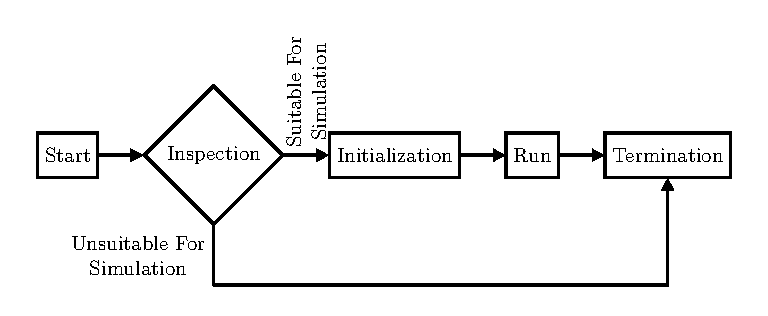
\includegraphics[width=\linewidth]{figures/FlowChart/flowchart.pdf}
    \caption{Flowchart of the simulation stages.}
    \label{fig: flowchart}
\end{figure}

\begin{figure}
    \centering
    \subfloat[]{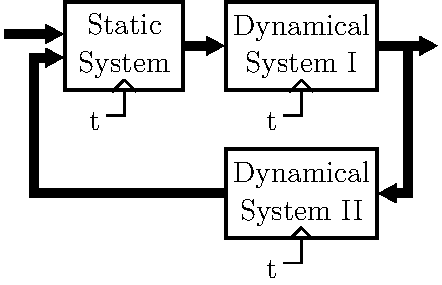
\includegraphics[width=0.49\linewidth]{figures/AlgebraicLoop/unbrokenloop.pdf} \label{subfig: unbroken algebraic loop}}
    \subfloat[]{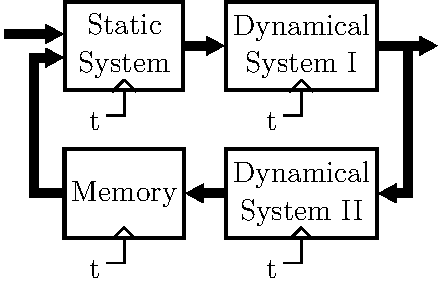
\includegraphics[width=0.49\linewidth]{figures/AlgebraicLoop/brokenloop.pdf} \label{subfig: broken algebraic loop}}
    \caption{\protect\subref{subfig: unbroken algebraic loop} An algebraic loop consisting of the components Static System, Dynamical System I and Dynamical System II. \protect\subref{subfig: broken algebraic loop} Breaking of the loop with a Memory component. }
    \label{fig: algebraic loop}
\end{figure}

In the \textit{inspection} stage, the model is inspected to see whether the model is suitable for simulation. If connections having any unconnected terminals are detected, the simulation is terminated at this stage. The model is not suitable for simulation when algebraic loops exist\cite{lamego2001adaptive}. An algebraic loop is a closed-loop consisting of one or more components whose outputs are directly dependent on their inputs. Almost every system that includes feedbacks has algebraic loops. The simulation does not proceed because none of the components in the loop can generate output to break the loop. Such a problem can be solved by redesigning the model so that the model has no algebraic loops, solving the feed-forward algebraic equation of the loop, or inserting a memory component with a particular initial condition anywhere in the loop. Causal.jl provides all these loop-breaking solutions. During the \textit{inspection}, when algebraic loops are detected, all the loops are broken, if possible, automatically. Otherwise, a report is printed to notify the user to insert memory components to break the loops.

\begin{figure}
    \centering
    \subfloat[]{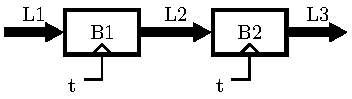
\includegraphics[width=0.5\linewidth]{figures/TaskForComponents/components.pdf} \label{subfig: components}} \\
    \subfloat[]{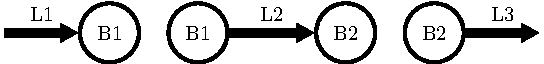
\includegraphics[width=.75\linewidth]{figures/TaskForComponents/tasks.pdf} \label{subfig: tasks}}
    \caption{Launching tasks for the connections. \protect\subref{subfig: components} An example model part consisting of the components B1 and B2 and the connections L1, L2 and L3. \protect\subref{subfig: tasks} Tasks launched corresponding to the connections.}
    \label{fig: tasks for components}
\end{figure}

If the model passes the \textit{inspection}, the writer and reader tasks are launched in the \textit{initialization} stage to ensure the data flow through the model connections. At this point, a writer and a reader task are bound to each connection. In Figure \ref{subfig: components} model part consisting of components B1, B2, and the connections L1, L2, L3 are shown. When triggered, the B1 reads data from L1, calculates its output, and writes to L2. Similarly, when triggered, B2 reads data from the L2, calculates its output, and writes to the L3. The tasks bounded to L1, L2, and L3 corresponding to B1 and B2 are shown in Figure \ref{subfig: tasks}. Since B1 reads the data from L1 and writes data to L2, a reader task is bounded to L1, and a writer task is bounded L2. Similarly, since B2 reads the data from L2 and writes data to L3, a reader task is bounded to L2, and a writer task is bounded L3. Since both a writer and a reader task are bound to the L2, data can flow from B1 to B2 through L2. A task manager is constructed to check whether the tasks launched during the \textit{initialization} are running correctly throughout the simulation.

The \textit{initialization} is followed by the \textit{run} stage. The tasks that are launched corresponding to the components during the \textit{initialization} expect the components to be triggered through their trigger pins. These triggers are generated in the sampling instants by the model clock during the \textit{run} stage. It is possible to sample the signals flowing through the connections at equal or independent time intervals. The generated triggers are put into the trigger pins of the components.

When the \textit{run} stage is completed, the tasks launched at the \textit{initialization} stage are closed in the \textit{termination} stage and the simulation ends.

The sampled values are interpolated for a duration of one sampling period so that the components can evolve independently. The sampling period is an essential factor that affects the accuracy of the simulation results directly.

\section{Illustrative Examples}

\subsection{Simulation of Models Having Different Component Types}
\begin{figure}
    \centering
    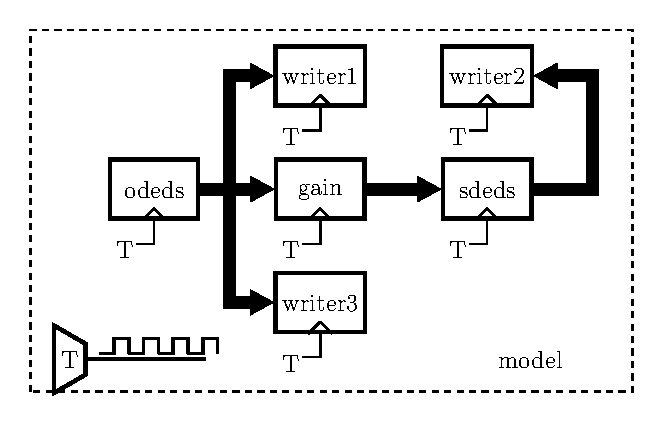
\includegraphics[width=\linewidth]{figures/CoupledChuaModel/coupled_chua_model.pdf}
    \caption{A model consisting of components represented by different equation types.}
    \label{fig: coupled model}
\end{figure}

In Causal.jl, it is possible to simulate models that include components represented by different types of equations. In Figure \ref{fig: coupled model} is given such an example model.`odeds` is a dynamical system represented by the ordinary differential equation in (\ref{eq: coupled ode}) where where $x_1, y_1, z_1$ are the state variables and $a=35, b=3, c = 28$ are system parameters.
\begin{equation}
    \begin{split}
        \dot{x}_1 &= a (y_1 - x_1) \\
        \dot{y}_1 &= (c - 1) x_1 + c y_1 - x_1 z_1 \\
        \dot{z}_1 &= x_1 y_1 - b z_1
    \end{split}
    \label{eq: coupled ode}
\end{equation}
`sdsds` is dynamical system that is represented by the stochastic differential equation in (\ref{eq: coupled sde}) where $x_2, y_2, z_2$ are the state variables, $u=[u_1,u_2, u_3]$ is the input, $\eta$ is noise strength, $W_t$ is the Wiener process corresponding to the noise and $a, b, c$ are the same as those in (\ref{eq: coupled ode}).
\begin{equation}
    \begin{split}
        dx_2 &= (a (y_1 - x_1) + u_1) dt + \eta dW_t \\
        dy_2 &= ((c - 1) x_1 + c y_1 - x_1 z_1)dt + \eta dW_t \\
        dz_2 &= (x_1 y_1 - b z_1 + u_3) dt + \eta dW_t 
    \end{split}
    \label{eq: coupled sde}
\end{equation}
`gain` is a static system whose input output relation is given in (\ref{eq: gain}) where $u, y, \epsilon$ are the input, output and gain coefficient of the system. 
\begin{equation}
    y = \epsilon u
    \label{eq: gain}
\end{equation}
`writer1` and `writer2` are used to record the outputs of `odeds` and `sdeds`, respectively, while `writer3` is used to record the fast Fourier transform(FFT) of the data flowing out of `odeds`\cite{proakis2004digital}. 

Being a domain-specific-language, Causal.jl provides a syntax for handy model construction. The program written using Causal.jl to construct and simulate the model in Figure \ref{fig: coupled model} is given in Listing \ref{lst: coupled codes}. The program first starts with the type definitions of the components `odeds`, `sdeds`, and `gain`, together with their fields' default values. Note that the types of components are defined as subtypes of the corresponding abstract component types, which shows how the user-defined component types can enrich the standard library of Causal.jl. `writer1` and `writer2` are used directly to record the data without further processing, so they do not need additional data processing plugins.
On the other hand, rather than directly recording the data, `writer3` is used to process the data online, so it needs an additional plugin. `FFTPlug` is defined for this purpose, and `writer3` is equipped with an instance. For the sake of this example, we used the `fft` function \cite{fftw}. The model is constructed and simulated for $100$ seconds with a step size of $0.001$ seconds. After the simulation, the data in `write1` and `writer2` are read back and plotted in Figure \ref{fig: coupled simulation results}. From Figure \ref{subfig: coupled simulation sde}, the presence of the noise is apparent in the trajectory of `sdeds`. 

The individual evolution of components makes it possible to simulate such models that include components represented by different equations. 

Causal.jl adopts a causal modeling approach in which the data flow through the connections is unidirectional. Components that write data to a connection drives other components that read data from the same connection. Thus, the topological structure of a model can be extracted by following the components that read data from the connections bound to the output ports of model components.

The order in which the connections are specified is arbitrary. One does not need to follow the true data flow directions through the connections. Therefore, complex topologies with many components can be defined concisely.

\begin{figure}
    \centering
    \subfloat[]{
        \begin{tikzpicture}
            \node[](plt){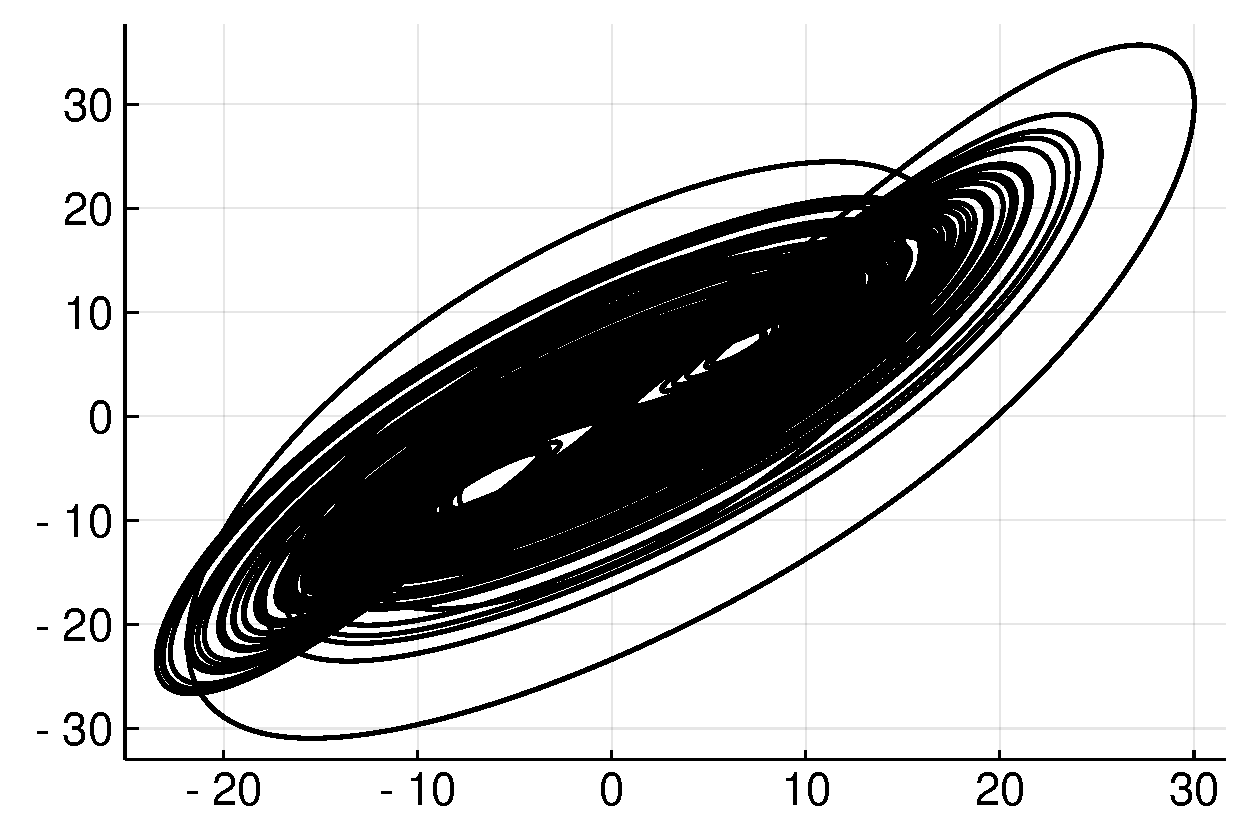
\includegraphics[scale=0.25]{figures/ChenSystemSimulations/odeds.pdf}};
            \node[] at (plt.south) {$x_1$};
            \node[] at (plt.west) {$y_1$};
        \end{tikzpicture}
        \label{subfig: coupled simulation ode}
        }\\
    \subfloat[]{
        \begin{tikzpicture}
            \node[](plt){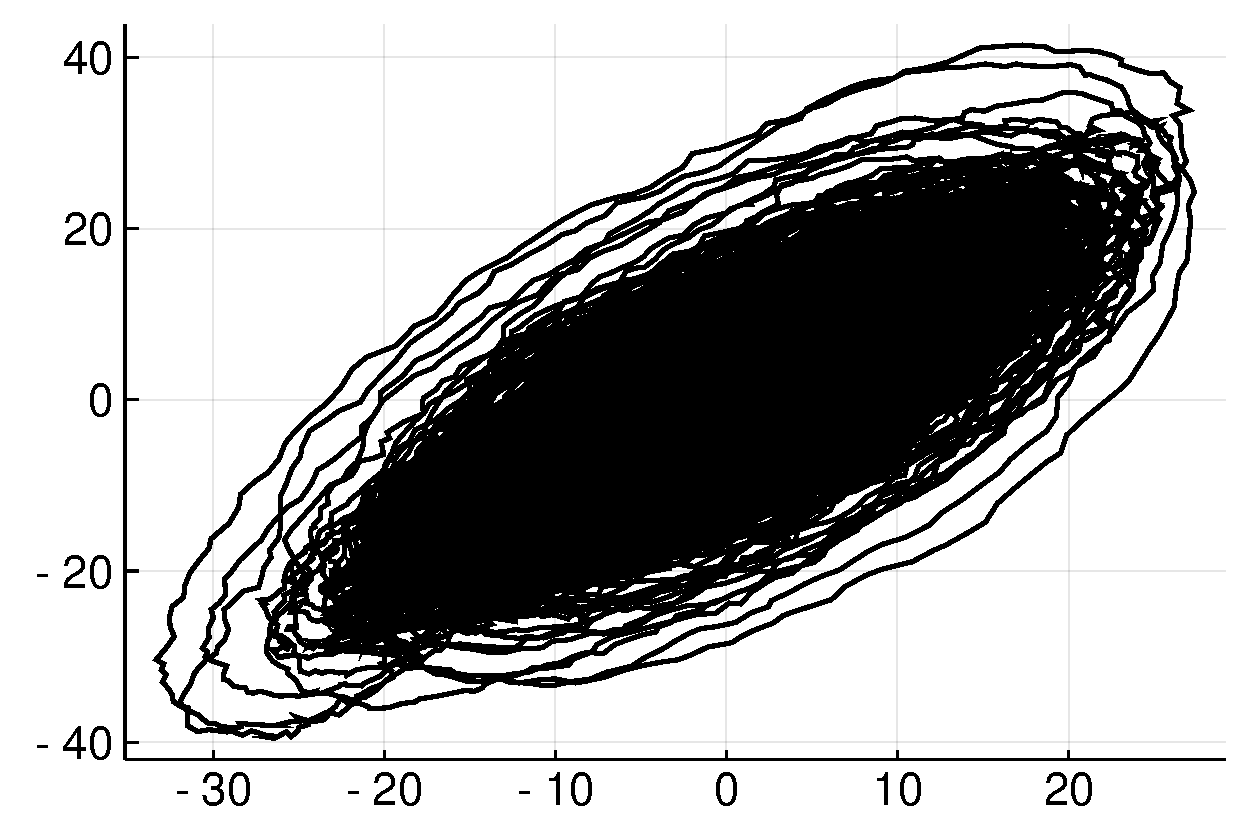
\includegraphics[scale=0.25]{figures/ChenSystemSimulations/sdeds.pdf}};
            \node[] at (plt.south) {$x_2$};
            \node[] at (plt.west) {$y_2$};
            \end{tikzpicture}
        \label{subfig: coupled simulation sde}
    }
    \caption{\protect\subref{subfig: coupled simulation ode} $x_1 - y_1$ trajectory of `odeds`. \protect\subref{subfig: coupled simulation sde} $x_2 - y_2$ trajectory of `sdeds`.}
    \label{fig: coupled simulation results}
\end{figure}

\subsection{Simulation of Models Consisting of a Large Number of Nodes}
In Causal.jl, its is possible to simulate large scale complex models consisting of a large number of dynamical system nodes. As an example, a network of continuous time identical dynamical systems is given Figure \ref{fig: network graph}. The nodes of the network evolve by 
\begin{equation}
    \dot{\bm{x}}_i = f(\bm{x}_i) + \bm{u}_i, \quad i = 1, \ldots, n
    \label{eq: network equation}
\end{equation}
where 
\begin{equation}
    \bm{u}_i = \sum_{i = 1}^n \epsilon_{ij} \bm{P} \bm{x}_j, \quad i = 1, \ldots, n,
    \label{eq: network node inputs}
\end{equation}
$n$ is the number of nodes, $\bm{x}_i \in \mathbb{R}^d$ is the state vector of node $i$, $f: \mathbb{R} \mapsto \mathbb{R}^d$ is the function corresponding to the individual node dynamics, $\epsilon_{ij} \geq 0 $ is the coupling strength between the nodes $i$ and $j$. The diagonal matrix $\bm{P} = diag(p_1, \ldots, p_d)$ determines by which state variables the nodes are connected to each other. The matrix $\bm{E} = [\epsilon_{ij}] \in \mathbb{R}^{n, n}, \; \epsilon_{ij} = \epsilon_{ji} \geq 0, \; \sum_{j = 1}^n \epsilon_{ij} = 0, i = 1, \ldots, n$ determines the network topology: if $\epsilon_{ij} > 0$, there is a connection between the nodes $i$ and $j$, if $\epsilon_{ij} = 0$, there is no connection between the nodes $i$ and $j$.

In the network given in Figure \ref{fig: network graph}, $n=50$,  $f$ is the Lorenz dynamics given by,
\begin{equation}
    \begin{split}
        \dot{x}_{i,1} &= \sigma (x_{i, 2} - x_{i, 1}) \\
        \dot{x}_{i,2} &= x_{i, 1} (\rho -  x_{i, 3}) - x_{i, 2} \\
        \dot{x}_{i,3} &= x_{i, 1} x_{i, 2} - \beta x_{i, 3}
    \end{split}
\end{equation}
where $\sigma=10, \beta=8/3, \rho=28$ are system parameters, $\bm{P} = diag(1, 0, 0)$. The network has Wattz-Strogatz topology that has a vertex degree of $10$ and that is randomized with a probability of $0.5$\cite{watts1998collective}.

\begin{figure}
    \centering
    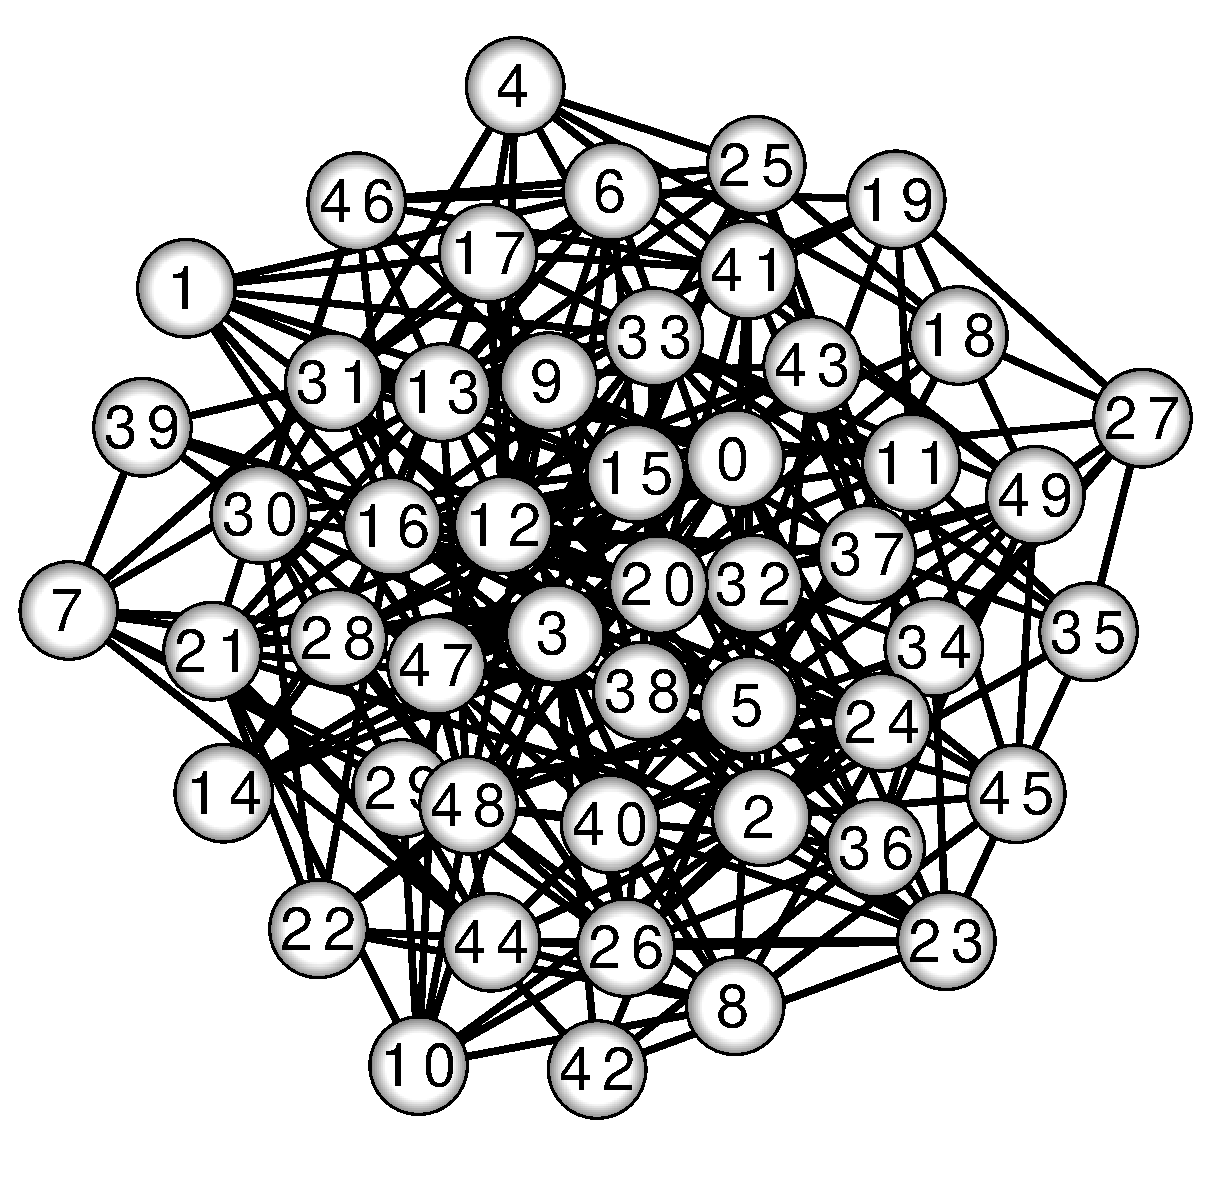
\includegraphics[width=0.5\linewidth]{figures/Networks/wattz_strogatz.pdf}    
    \caption{A network consisting of identical dynamical system nodes The spheres and the line segments represent the dynamical system nodes and the connection between them, respectively.}
    \label{fig: network graph}
\end{figure}

The model in Figure \ref{fig: network graph} is given in Figure \ref{fig: network model}. `node $k$` for $k =1, \ldots, n$ correspond to the dynamical system nodes of the network.  From (\ref{eq: network equation}) and (\ref{eq: network node inputs}), we see that the states of the nodes are taken as their outputs, weighted by the coupling strengths and fed back to their inputs. Hence, `coupler` is used to construct the weighted outputs. `writer` records the nodes' outputs. The model has algebraic loops $L_k$ for $k = 1, \ldots, n$, where the algebraic loop $L_k$ consists of `node $k$` and `coupler`. 

\begin{figure}
    \centering
    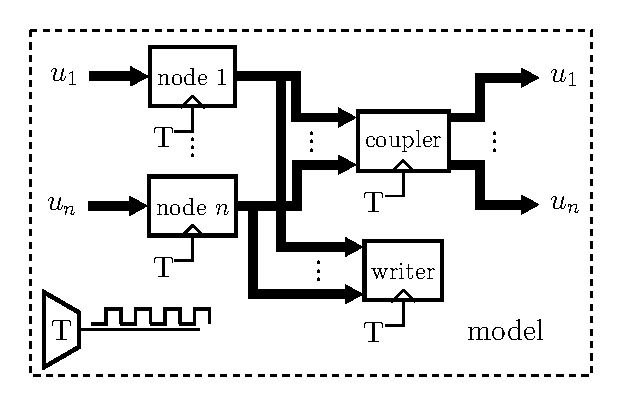
\includegraphics[width=0.8\linewidth]{figures/NetworkModel-WattzStrogatz/network_wattz_strogratz.pdf}
    \caption{Block diagram model of the network in Figure \ref{fig: network graph}.}
    \label{fig: network model}
\end{figure}

The program written using Causal.jl to construct and simulate the model in Figure \ref{fig: network model} is given in Listing \ref{lst: network codes}. Having defined the types of dynamical system nodes and the coupler, the model is constructed and simulated for $100$ seconds with a sampling period of $0.005$ seconds. After the simulation, the simulation data is read back from the writer and the mean square error (MSE) 
\begin{equation}
    MSE(t) = \dfrac{1}{n} \sum_{i = 2}^n \Vert \bm{x}_{1,1}(t) - \bm{x}_{i,1}(t) \Vert
\end{equation}
is computed and plotted. It is seen from Figure \ref{subfig: network error} that the all the nodes in the network synchronize with each other as the MSE goes to zero as time evolves. 

Note from the program in Listing \ref{lst: network codes} that memory components are not used to break algebraic loops of the model. Causal.jl is capable of detecting and breaking these algebraic loops automatically without requiring any user intervention. 

\begin{figure}
    \centering
    \subfloat[]{
        \begin{tikzpicture}
            \node[](plt){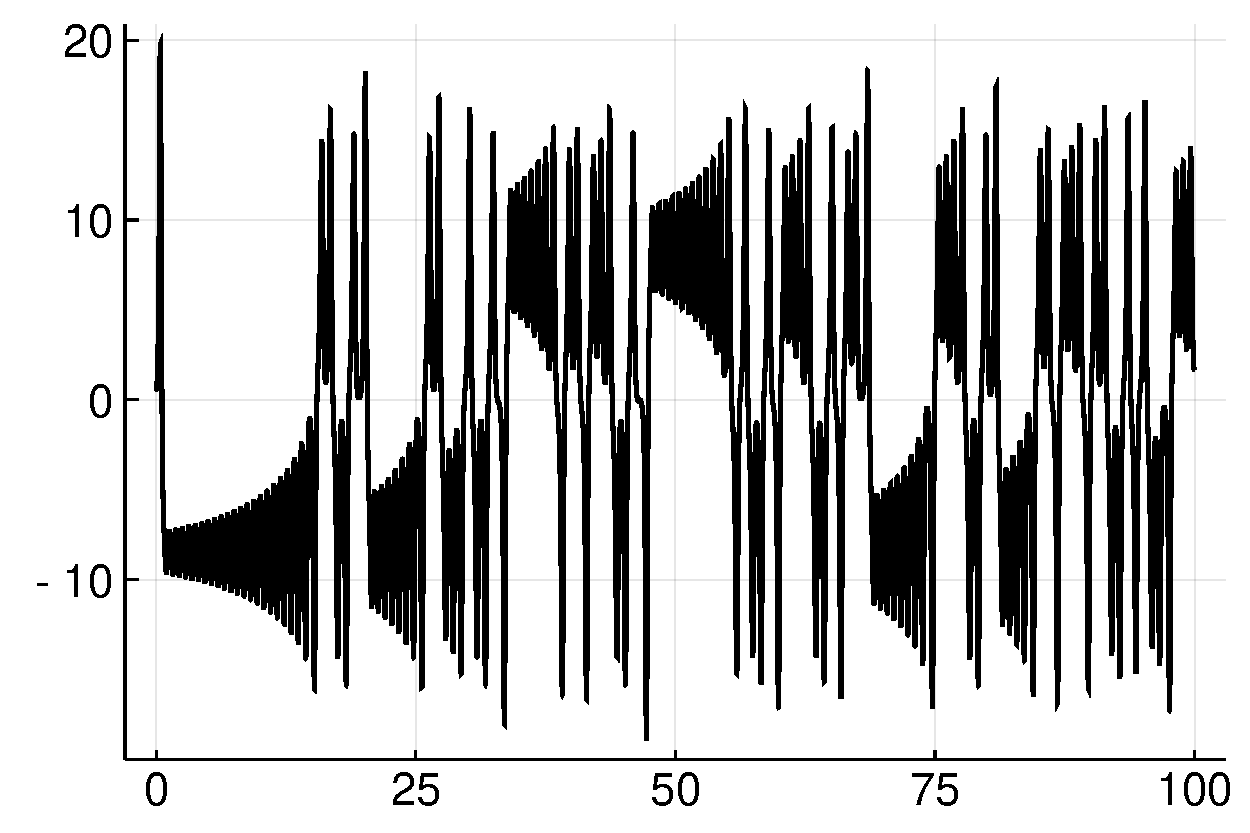
\includegraphics[scale=0.25]{figures/NetworkSimulation-WattzStrogatz/waveform.pdf}};
            \node[] at (plt.south) {$t$ [seconds]};
            \node[] at (plt.west) {$x_{1,1}$};
        \end{tikzpicture}
        \label{subfig: network timewaveform}
        }\\[-0.1cm]
    \subfloat[]{
        \begin{tikzpicture}
            \node[](plt){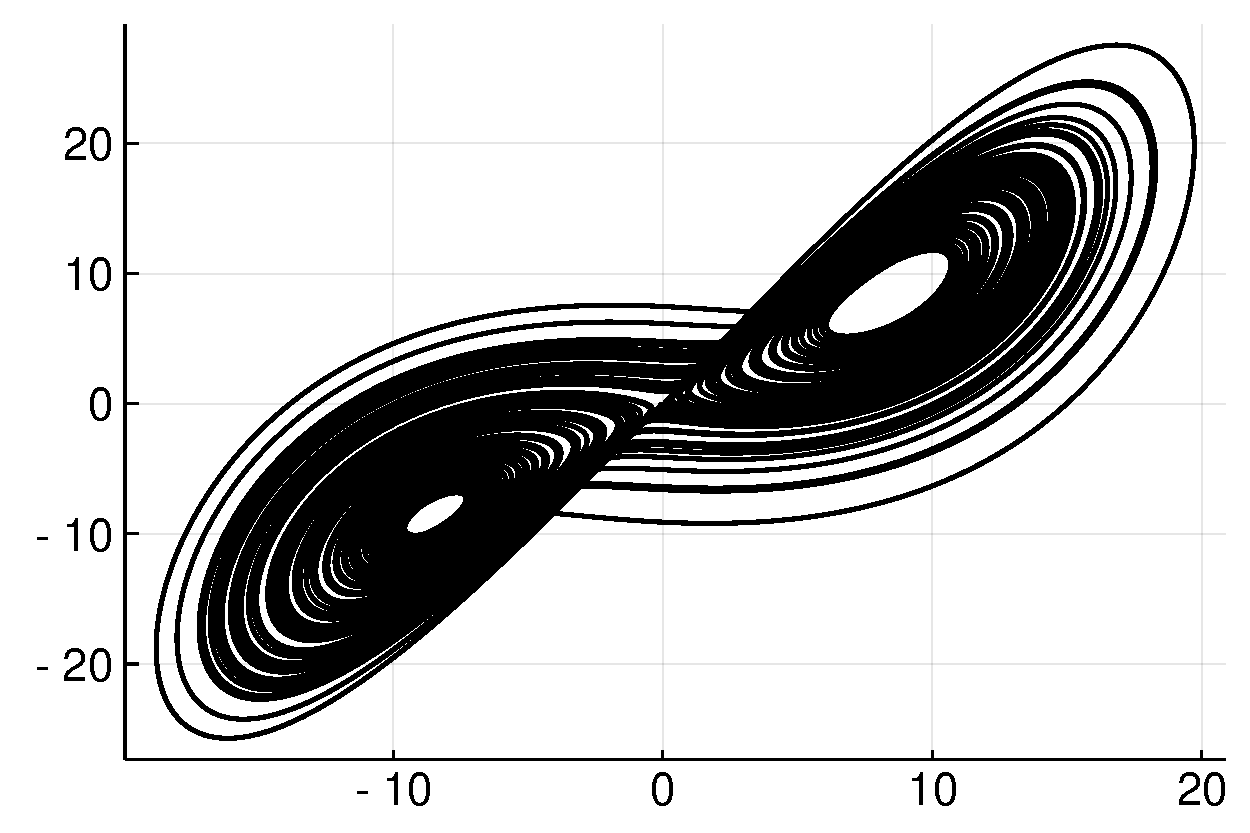
\includegraphics[scale=0.25]{figures/NetworkSimulation-WattzStrogatz/trajectory.pdf}};
            \node[] at (plt.south) {$x_{1,1}$};
            \node[] at (plt.west) {$x_{1, 2}$};
            \end{tikzpicture}
        \label{subfig: network trajectory}
    } \\[-0.1cm]
    \subfloat[]{
        \begin{tikzpicture}
            \node[](plt){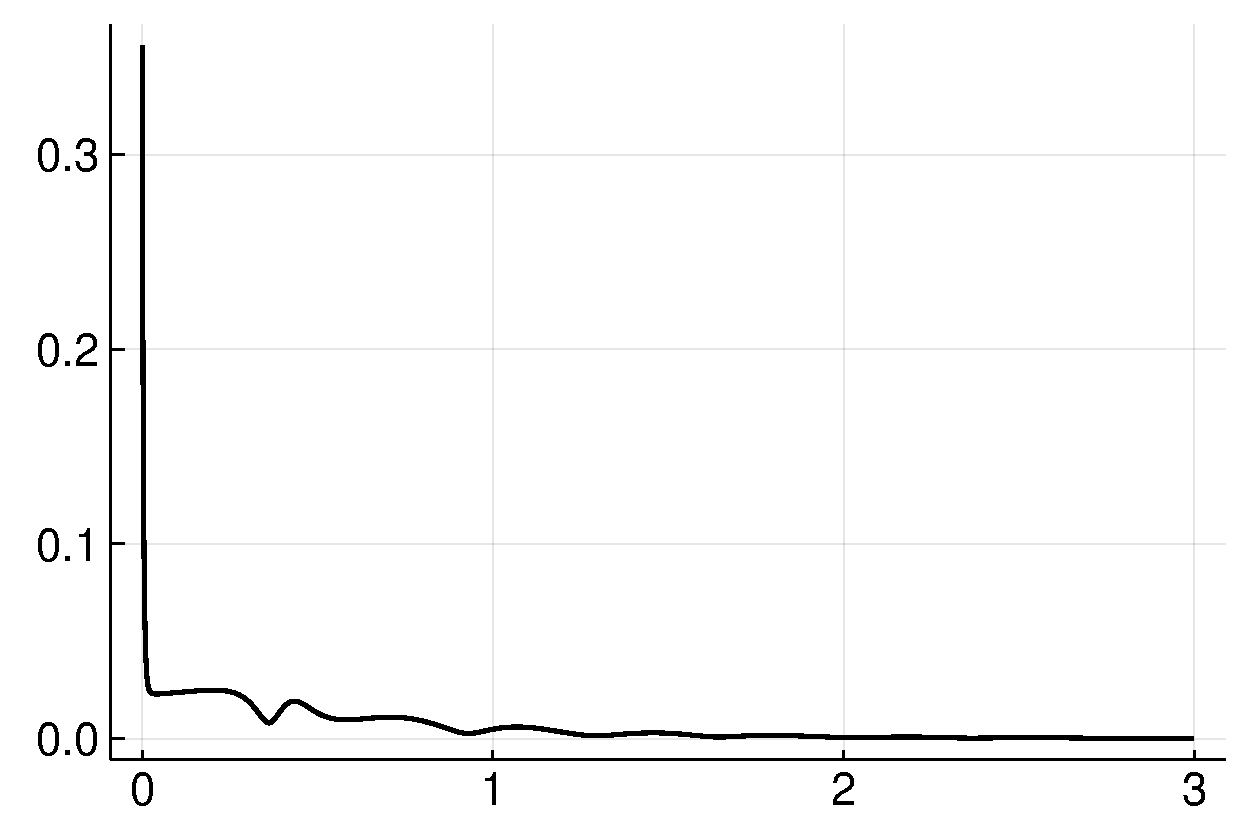
\includegraphics[scale=0.25]{figures/NetworkSimulation-WattzStrogatz/error.pdf}};
            \node[] at (plt.south) {$t$ [seconds]};
            \node[xshift=-0.25cm] at (plt.west) {MSE};
            \end{tikzpicture}
        \label{subfig: network error}
    }
    \caption{Simulation results the model given in Figure \ref{fig: network model}. \protect\subref{subfig: network timewaveform} Time waveform of $x_{1,1}$. \protect\subref{subfig: network trajectory} $x_{1,1} - x_{1,2}$ trajectory. \protect\subref{subfig: network trajectory} MSE.}
    \label{fig: network simulation results}
\end{figure}

\section{Conclusion}
In this paper, we introduced Causal.jl. In Causal.jl, the simulation is performed by evolving the components according to their mathematical equations between the sampling intervals in parallel and independently. The components can be static or dynamical or represented by mathematical equations having continuous or discrete-time variables. The simulation of the models consisting of components defined by ordinary, random ordinary, stochastic, delay differential, differential-algebraic, or difference equations is possible. It is not an obligation to describe all the model components with the same type of mathematical equation.

The data flowing through the connections can be directly recorded or visualized during the simulation. In addition to the offline analyzes, with user-defined plugins, it is also possible to carry out online data analysis such as extracting statistical or spectral properties, applying different signal processing techniques, etc. 

The model components evolve in parallel and simultaneously. The tasks of the Julia programming language is used for this parallel evolution. The tasks allow switching between the evolution of the components during the simulation. Using the Julia programming language's distributed computing tools, it is possible to distribute computation workload on multiple processors.

Especially when considering extensive system networks consisting of thousands of system nodes, it is an important advantage that the system models can be created easily and quickly, that such models can be simulated in multiple microprocessor cores with distributed programming tools and that the proposed tool can provide this with an easy syntax.

\section{Acknowledgements}
This work was supported by Scientific Research Projects Funding Program of Dokuz Eylül University (project no: 2020.KB.FEN.007).

% **************GENERATED FILE, DO NOT EDIT**************

\bibliographystyle{juliacon}
\bibliography{ref.bib}


\onecolumn
\appendix 

\begin{lstlisting}[caption={Program using Causal.jl for the simulation of the system in Figure \ref{fig: coupled model}. Plots.jl is used to plot the simulation data while FFTW.jl is used to compute the FFT of the simulation data \cite{plots, fftw}.}, label={lst: coupled codes}, language=Julia]
using Causal, Plots, FFTW

# Define ODE system type under AbstractODESystem
@def_ode_system mutable struct ODESys{RH, RO, IP, OP} <: AbstractODESystem
    righthandside::RH = function fode(dx, x, u, t, a=35., b=3., c=28.)
        dx[1] = a * (x[2] - x[1])
        dx[2] = (c - a) * x[1] + c * x[2] - x[1] * x[3]
        dx[3] = x[1] * x[2] - b * x[3]
    end
    readout::RO = (x, u, t) -> x 
    state::Vector{Float64} = rand(3)
    input::IP = nothing
    output::OP = Outport(3)
end

# Define SDE system type under AbstractSDESystem
@def_sde_system mutable struct SDESys{DR, DF, RO, IP, OP} <: AbstractSDESystem
    drift::DR = function fsde(dx, x, u, t, a=35., b=3., c=28.)
        dx[1] = a * (x[2] - x[1]) + u[1](t)
        dx[2] = (c - a) * x[1] + c * x[2] - x[1] * x[3] + u[2](t)
        dx[3] = x[1] * x[2] - b * x[3] + u[3](t)
    end
    diffusion::DF = (dx, x, u, t, η=10.) -> (dx .= η) 
    readout::RO = (x, u, t) -> x
    state::Vector{Float64} = rand(3)
    input::IP = Inport(3)
    output::OP = Outport(3)
end

# Define Gain system type under AbstractStaticSystem
@def_static_system struct GainSys{RO,IP,OP} <: AbstractStaticSystem 
    readout::RO = (u,t, ϵ=0.1) -> ϵ * u 
    input::IP = Inport(3)
    output::OP = Outport(3)
end 

# Define plugin type under AbstractPlugin
@def_plugin struct FFTPlug{PR} <: AbstractPlugin 
    process::PR = x -> fft(x, 2)    # Computes FFT of the data `x`
end 

# Construct model
@defmodel model begin 
    @nodes begin 
        odeds = ODESys()    # Add odeds component  
        gain = GainSys()    # Add gain  component   
        sdeds = SDESys()    # Add sde components
        writer1 = Writer(input=Inport(3))                   # Add writer without plugin
        writer2 = Writer(input=Inport(3))                   # Add writer without plugin
        writer3 = Writer(input=Inport(3), plugin=FFTPlug()) # Add writer with `FFTPlug` plugin
    end
    @branches begin 
        odeds => gain       # Add connection from `odeds` to `gain`.
        gain => sdeds       # Add connection from `gain` to `sdeds`.
        odeds => writer1    # Add connection from `odeds` to `writer1`.
        sdeds => writer2    # Add connection from `sdeds` to `writer2`.
        odeds => writer3    # Add connection from `odeds` to `writer3`.
    end 
end 

# Simulate model 
sim = simulate!(model, 0, 0.001, 100) # Simulate from 0 to 100 seconds with a step size of 0.001 seconds

# Plot simulation data 
t, x1 = read(getnode(model, :writer1).component)
t, x2 = read(getnode(model, :writer2).component)
x3 = read(getnode(model, :writer3).component, flatten=false)
plot(x1[:, 1], x1[:, 2], subplot=1, label="")
plot(x2[:, 1], x2[:, 2], subplot=2, label="")   
println(x3)  
\end{lstlisting}

\begin{lstlisting}[caption={Program using Causal.jl for the simulation of the system in Figure \ref{fig: network graph}. Plots.jl is used to plot the simulation data while LightGraphs.jl is used to construct the connectiviy matrix of the network topology \cite{plots, lightgraphs}}, label={lst: network codes}, language=Julia]
using Causal, Plots
using LightGraphs: watts_strogatz, laplacian_matrix

# Define DynamicSystem type under AbstractODESystem
@def_ode_system mutable struct DynamicSystem{RH, RO, IP, OP} <: AbstractODESystem
    righthandside::RH = function f(dx, x, u, t, σ=10., β=8/3, ρ=28)
        dx[1] = σ * (x[2] - x[1]) + u[1](t)
        dx[2] = x[1] * (ρ - x[3]) - x[2] + u[2](t)
        dx[3] = x[1] * x[2] - β * x[3] + u[3](t)
    end
    readout::RO = (x, u, t) -> x
    state::Vector{Float64} = rand(3)
    input::IP = Inport(3)
    output::OP = Outport(3) 
end  

# Define Coupler type under AbstractStaticSystem
@def_static_system struct CouplerSystem{ET, CT, IP, OP, RO} <: AbstractStaticSystem
    E::ET
    P::CT
    input::IP = Inport(size(E, 1) * size(P, 1))
    output::OP = Outport(size(E, 1) * size(P, 1))
    readout::RO =  (u, t, E=E, P=P) ->  kron(E, P) * u
end

# Construct network parameters 
n = 50      # Number of nodes 
d = 3       # Dimension of each node
ϵ = 20.     # Coupling strength 
components = [DynamicSystem() for i in 1 : n]
E = ϵ * collect(-laplacian_matrix(watts_strogatz(n, 10, 0.5)))  # Connectivity matrix of network topology
P = [1 0 0; 0 0 0; 0 0 0]   # Systems are coupled by their first state variable.

# Construct model 
model = Model() 

# Add components
for (i, component) in enumerate(components)
    addnode!(model, component, label=Symbol("node$i"))
end
addnode!(model, CouplerSystem(E=E, P=P), label=Symbol("coupler"))
addnode!(model, Writer(input=Inport(n * d)), label=Symbol("writer"))

# Add connections
m = n + 1
for (j, k) in zip(1:n, map(i -> i : i + d - 1, 1 : d : n * d))
    addbranch!(model, j => m, 1 : d => k)
    addbranch!(model, m => j, k => 1 : d)
end
p = n + 2
for (j, k) in zip(1:n, map(i -> i : i + d - 1, 1 : d : n * d))
    addbranch!(model, j => p, 1 : d => k)
end

# Simulate model 
sim = simulate!(model, 0, 0.001, 100.)

# Read and plot the simulation data 
t, x = read(getnode(model, :writer).component)

# Compute mean square error
mse = sqrt.(sum(diff(x[:, 1 : d : end],dims=2).^2/n, dims=2))

# Plot results
k = 3000 
plot(t, x[:, 1] , label="")
plot(x[:, 1], x[:,2], label="")
plot(t[1:k], mse[1:k], label="")
\end{lstlisting}

\end{document}

% Inspired by the International Journal of Computer Applications template
